\documentclass[11pt]{article}

%  USE PACKAGES  ---------------------- 
\usepackage[margin=0.7in,vmargin=1in]{geometry}
\usepackage{amsmath,amsthm,amsfonts}
\usepackage{amssymb}
\usepackage{fancyhdr}
\usepackage{enumerate}
\usepackage{mathtools}
\usepackage{hyperref,color}
\usepackage{enumitem,amssymb}
\usepackage{indentfirst}
\newlist{todolist}{itemize}{4}
\setlist[todolist]{label=$\square$}
\usepackage{pifont}
\newcommand{\cmark}{\ding{51}}%
\newcommand{\xmark}{\ding{55}}%
\newcommand{\done}{\rlap{$\square$}{\raisebox{2pt}{\large\hspace{1pt}\cmark}}%
\hspace{-2.5pt}}
\newcommand{\HREF}[2]{\href{#1}{#2}}
\usepackage{textcomp}
\usepackage{listings}
\lstset{
basicstyle=\small\ttfamily,
% columns=flexible,
upquote=true,
breaklines=true,
showstringspaces=false
}
%  -------------------------------------------- 

%  HEADER AND FOOTER (DO NOT EDIT) ----------------------
\newcommand{\problemnumber}{0}
\pagestyle{fancy}
\fancyhead{}
%\fancyhead[L]{\textbf{Question \problemnumber}}
\newcommand{\newquestion}[1]{
\clearpage % page break and flush floats
\renewcommand{\problemnumber}{#1} % set problem number for header
\phantom{}  % Put something on the page so it shows
}
\fancyfoot[L]{IE 332}
\fancyfoot[C]{Project submission}
\fancyfoot[R]{Page \thepage}
\renewcommand{\footrulewidth}{0.4pt}

%  --------------------------------------------


%  COVER SHEET (FILL IN THE TABLE AS INSTRUCTED IN THE ASSIGNMENT) ----------------------
\newcommand{\addcoversheet}{
\clearpage
\thispagestyle{empty}
\vspace*{0.5in}

\begin{center}
\Huge{{\bf IE332 Project \#2}} % <-- replace with correct assignment #

Due: April 28th, 11:59pm EST % <-- replace with correct due date and time
\end{center}

\vspace{0.3in}

\noindent We have {\bf read and understood the assignment instructions}. We certify that the submitted work does not violate any academic misconduct rules, and that it is solely our own work. By listing our names below we acknowledge that any misconduct will result in appropriate consequences. 

\vspace{0.2in}

\noindent {\em ``As a Boilermaker pursuing academic excellence, I pledge to be honest and true in all that I do.
Accountable together -- we are Purdue.''}

\vspace{0.3in}

\begin{table}[h!]
  \begin{center}
    \label{tab:table1}
    \begin{tabular}{c|ccc|c|c}
      Student & Research & Challenges & Report & Overall & DIFF\\
      \hline
      Natalie & 20 & 20 & 20 & 20 & 20\\
      Jakob & 20 & 20 & 20 & 20 & 20\\
      Jack & 20 & 20 & 20 & 20 & 20\\
      Alex & 20 & 20 & 20 & 20 & 20\\
      Kento & 20 & 20 & 20 & 20 & 20\\
      \hline
      St Dev & 0 & 0 & 0 & 0 & 0\\
    \end{tabular}
  \end{center}
\end{table}

\vspace{0.2in}

\noindent Date: \today.
}
%  -----------------------------------------

%  TODO LIST (COMPLETE THE FULL CHECKLIST - USE AS EXAMPLE THE FIRST CHECKED BOXES!) ----------------------
\newcommand{\addtodo}{
\clearpage
\thispagestyle{empty}

\section*{Read Carefully. Important!}

\noindent By electronically uploading this assignment to Brightspace you acknowledge these statements and accept any repercussions if in any violation of ANY Purdue Academic Misconduct policies. You must upload your homework on time for it to be graded. No late assignments will be accepted. {\bf Only the last uploaded version of your assignment before the due date will be graded}.

\vspace{0.2in}

\noindent {\bf NOTE:} You should aim to submit no later than 30 minutes before the deadline, as there could be last minute network traffic that would cause your assignment to be late, resulting in a grade of zero. 

\vspace{0.2in}

\noindent When submitting your assignment it is assumed that every student considers the below checklist, as there are grading consequences otherwise (e.g., not submitting a cover sheet is an automatic grade of ZERO).

\begin{todolist}

    \item[\done] Your solutions were prepared using the \LaTeX template provided in Brightspace. 
    \item[\done] Your submission has a cover sheet as its first page and this checklist as its second page, according to the template provided.
	 \item All of your solutions (program code, etc.) are included in the submission as requested. % Check this checkbox and the following ones if satisfied <---
    \item You have not included any screen shots, photos, etc. (plots should be intermediately saved as .png files and then added into your .tex file). % <---
	 \item All math notation and algorithms (algorithmic environment) are created using appropriate \LaTeX code (no pictures, handwritten solutions, etc.). % <---
    \item The .pdf is submitted as an individual file and not in a {\tt .zip}.
    \item You kept the \LaTeX source code in your files until this assignment is graded, in case you are required to show proof of creating your assignment using \LaTeX.  % <---
    \item If submitting with a partner, your partner is added in the submission section in Gradescope after you upload your file. % <---
    \item You have correctly matched each question to its page \# in the .pdf submission in the Gradescope section (after you uploaded your file).
    \item Watch videos on creating pseudocode if you need a refresher or quick reference to the idea. These are good starter videos:    % <---
    
     \HREF{https://www.youtube.com/watch?v=4jLO0vXPktU}{www.youtube.com/watch?v=4jLO0vXPktU} 
    
    \HREF{https://www.youtube.com/watch?v=yGvfltxHKUU}{www.youtube.com/watch?v=yGvfltxHKUU}
\end{todolist}
}

%% LaTeX
% Für alle, die die Schönheit von Wissenschaft anderen zeigen wollen
% For anyone who wants to show the beauty of science to others

%  -----------------------------------------


\begin{document}


\addcoversheet
\addtodo

% BEGIN YOUR ASSIGNMENT HERE:
\newpage
\tableofcontents

% Algorithm Research
\newpage
\section{Sub-Algorithm Research}

%sub-algorithm one
\subsection{Fast Gradient Sign Method}
With respect to adversarial attacks, the Fast Gradient Sign Method (FGSM) is one of the most popular and widely employed. This method was first theorized in 2015 by Stanford professor Ian J. Goodfellow and his colleagues in the paper EXPLAINING AND HARNESSING ADVERSARIAL EXAMPLES [ICLR 2015]. They noticed that the current neural networks are too linear and suggest that some cheap, yet analytical perturbations of the linear model can alter the neural networks. They came to this conclusion after analyzing the LSTMs, ReLUs, and maxout networks, which are all designed to work in linear, yet effective ways. \\

In order to fool our machine learning algorithm, the FGSM takes in three variables; the input image, the trained model, and epsilon. The first step is to take the input image (x), the parameters of the model (theta), and the targets associated with the input image (y) in order to compute J(theta, x, y). This is calculated with the means to linearize the function around the parameters of the model (theta). This will return the optimal max value of the vector (optimal max-norm). This max value of the vector is also known as the gradient, which will eventually be multiplied by epsilon and added to the image. Epsilon is a decimal value from zero to one which determines the magnitude of the perturbation on the gradient once added to the original image. Different epsilons lead to different confidence percentages. A higher epsilon does not mean a higher confidence percentage, therefore it is best to create a graph which will plot out the different epsilons with respect to the erroneous confidence percentages in order to find the optimal epsilon. Once the final image is created, we input the image into our model and finally get to see that the model has been fooled.

\begin{figure}[h]
\centering
\caption{A demonstration of a fast adversarial example where an imperceptibly small change is done to the original image in order to alter the final image and fool the training program. NOTE: Epsilon is equal to 0.007}
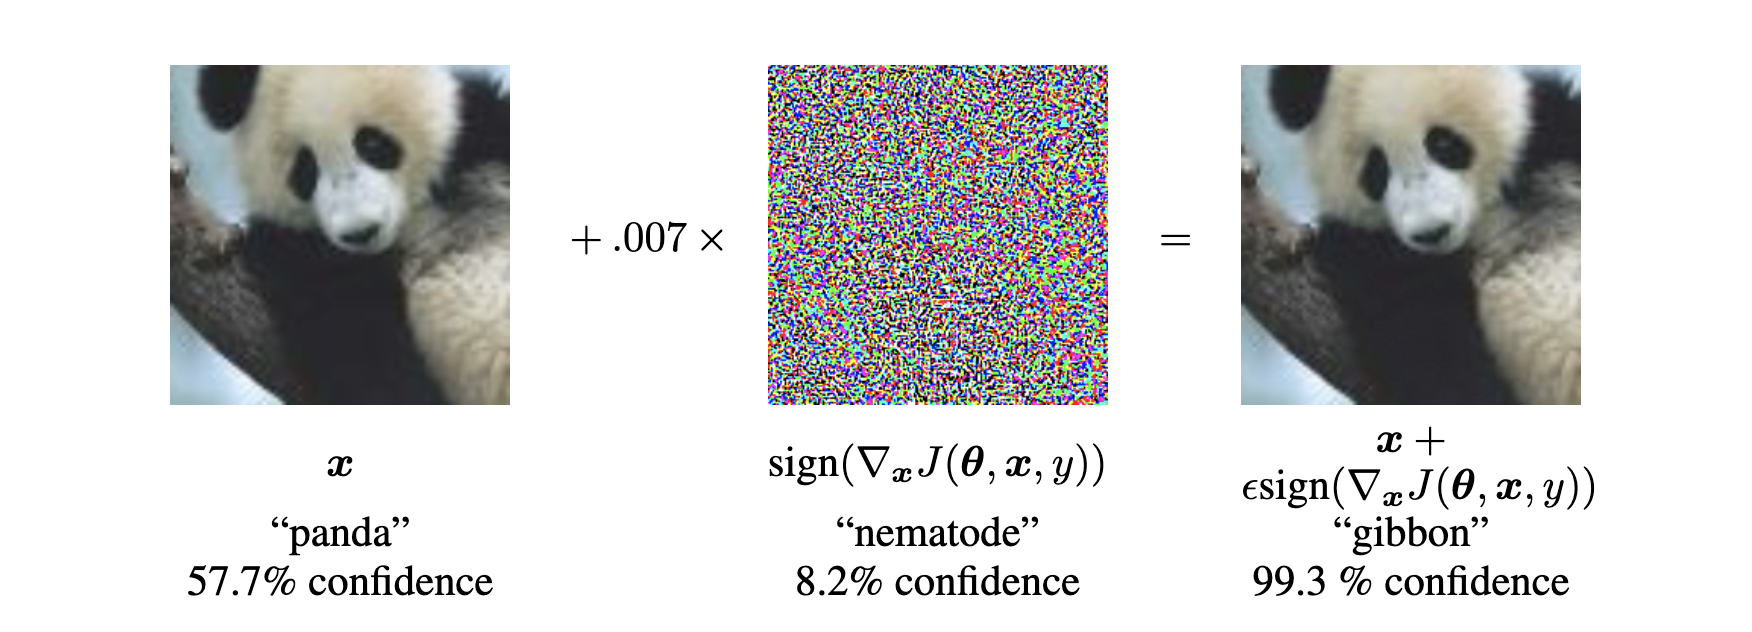
\includegraphics[height = 6.5cm]{FGSM_1.png}
\end{figure}

FGSM fools our machine classifier since it uses the trained model itself in order to compute the gradient by calculating the loss after propagation, essentially using the way the model works against itself. When the model tries reading the picture, it runs into a back-propagation issue regarding the way that it classifies the grass and the dandelions. These issues then lead to the misclassification of the inputs, which is our goal. One of the biggest advantages of this adversarial attack method when compared to others is that it is cheap and efficient. There are other methods, such as JBSM, which changes the image into a Jacobian Matrix in order to analyze the model’s reaction to each of the pixels. This can be rather time consuming and inefficient. It is also important to add that the linear nature of this algorithm leads to the economic and efficient aspect of this algorithm. This algorithm does have its weaknesses though, such as the fact that it is limited to linear models. This leads to a drop of efficiency with more complex algorithms. Another weakness with this algorithm is that it is vulnerable to being detected and prevented. This is because the actual image is being changed, although ever so slightly. Lastly, the simplicity of this algorithm means that it does not lead to the most efficient outcomes possible. In order to address these issues, there have been other versions of the FGSM, such as the Basic Iterative Method (BIM) and the Projected Gradient Descent (PGD).
\\
\\
In the context of our project, we would have taken 5 main steps:
\begin{enumerate}
\item Set a working directory and input the model using the load\_model\_tf().
\item Create a function called FGSM which takes in the model, x, y, and epsilon and returns the original image (x) with the gradient on it.
\item Create a for loop where every image in the "Dandelions" folder is uploaded into and turned into an array using the image\_to\_array() function. It also initializes an epsilon of 0.01.
\item Assign "model \%greater than\% predict(FGSM(model, x, y, e))" to a variable named "result". This uses the predict with respect to the model and the output of the function FGSM.
\item Print out the larger of the two percentages along with the name of the image file and run again with the folder containing the true "Grass" images.
\end{enumerate}

%sub-alorithm two
\subsection{L-BFGS} 
\par The L-BFGS method, or the Limited-Memory Broyden-Fletcher-Goldfarb-Shanno algorithm, was of interest to us in our research on performing adversarial attacks on image classifiers. Consistent with many other adversarial attack methods, L-BFGS would fool an image classifier by making small perturbations in an image.
\begin{figure}[h]
\centering
\caption{Simple L-BFSG attack with the purpose of making an image classifier think a 5 is some other number. The first row is the perturbed image, the second row is the perturbations that were added, and the third row is the original, unperturbed image. Here, the image has been fooled into misclassifying the 3 into a 4, a 6, and an 8, respectively.}
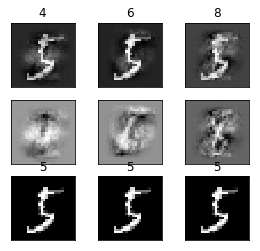
\includegraphics[height = 6.5cm]{l-bfsg 2.png}
\end{figure} \\
\par First, images are converted into arrays that contains all of the pixel values; these arrays are the input of the L-BFGS algorithm. The objective function of the algorithm is designed to minimize the function maximizing the likelihood of classifier misidentification; the minimax feature of this function is designed to preserve memory and improve runtime efficiency. The algorithm then changes the pixel parameters slightly and finds how the output of the image classifier is affected before iterating this process a certain number of times. The number of iterations can be defined by the user, or it could depend on some condition, like a percentage decrease in accuracy of the image classifier's predictions - in the case of our project, we would most likely implement a constraint for the algorithm to stop when the image classifier output a 49\% certainty on the correct classification of an image. \\
\par The iterations and the data obtained from them are then stored within the algorithm, and a Hessian matrix is produced from this information. The Hessian matrix is composted of second-order partial derivates that describe the behavior of every variable within an objective function. This matrix and its eigenvalues allow the model to understand how changing pixels within the training dataset affects the image classifier's output and apply this learning to images outside of the training set.
\begin{figure}[h]
\centering
\caption{Hessian Matrix Visualization. In large datasets, it is computationally impossible to calculate every eigenvalue in the Hessian matrix - here, a set of the smallest and largest eigenvalues have been produced to represent the importance of different pixels.}
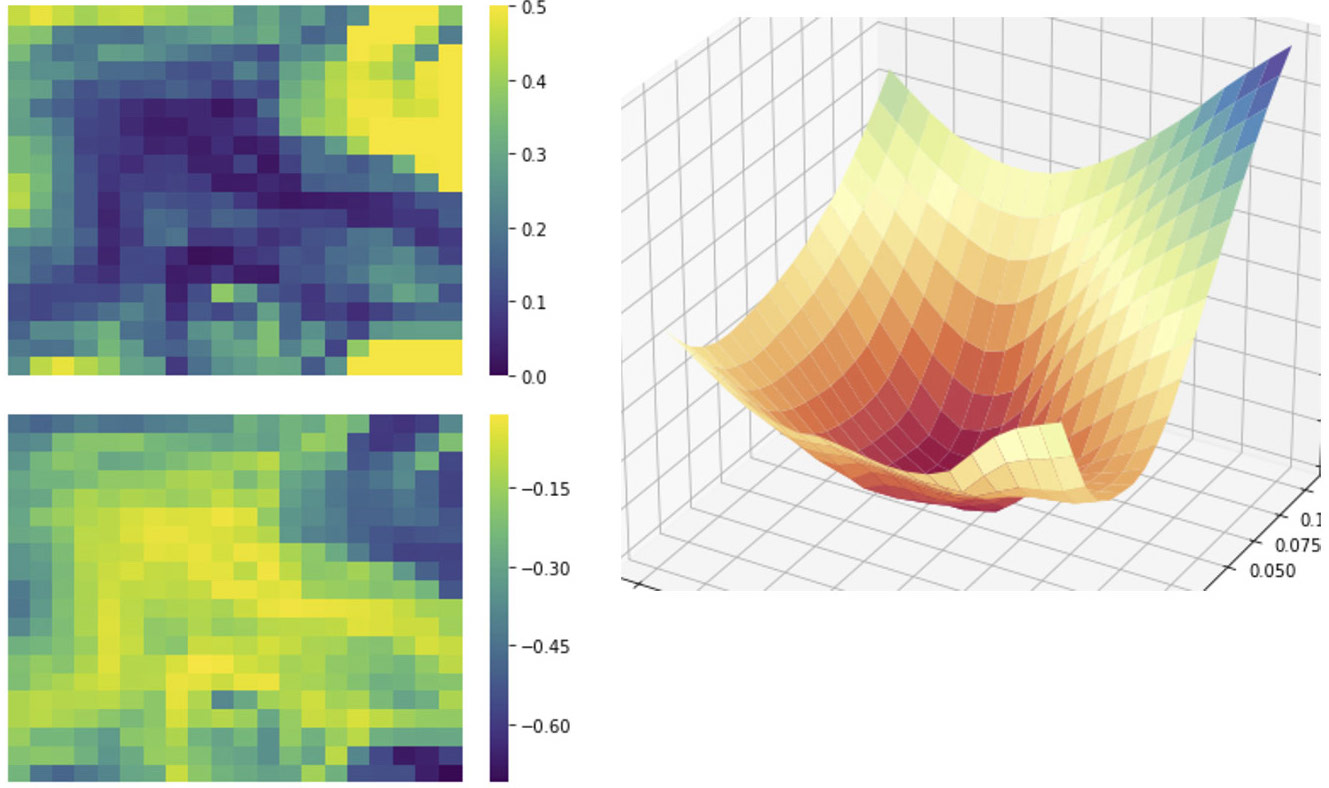
\includegraphics[height = 5cm]{hessianMatrix.jpeg}
\end{figure}
\par It is worth noting that the L-BFGS method is a variation of the original BFGS method, which is more computationally intensive. The BFGS method calculates the entire Hessian matrix and its relevant eigenvalues for every iteration of the algorithm, rather than completing a limited number of iterations and computing a Hessian matrix based off of those, making it less ideal for neural networks and deep learning networks that contain large amounts of information or devices with less computing power. \\
\par Lastly, the LP-BFGS (Limited-pixel Broyden-Fletcher-Goldfarb-Shanno) method is another, particularly compelling variation of the BFGS method that we explored in our research on adversarial attacks on image classifiers. Although it does not have a feature that limits the memory used, it could be especially applicable to the "pixel budget" factor of this project. The method of this algorithm is essentially the same as that of the BFGS and L-BFGS methods, but with one key difference: before the algorithm begins iterations to optimize the objective function, an integrated-gradient method is applied to the pixels within the image to first find which pixels are most important to the classifier's image recognition. The integrated-gradient method works by setting a sort of "baseline" that contains no data about the image classifier's predictions, or what pixels are deemed most important; then, as the model iterates through different pixels to see which ones are the most essential to image, data about the number of iterations, classification accuracy at the time of each iteration, and how much the classification accuracy was influenced are recorded over a pre-defined number of pixels. This will identify the most important pixels; finally, these pixels are then turned into variables within the objective function, and the algorithm begins its iterations to optimize the changes to just these pixels.
\newpage
\begin{figure}[h]
\centering
\caption{Visualization of the LP-BFGS method. Here, the integrated-gradient method has identified 4 pixels as the most important and used them as optimization variables in the objective function to perturb them.}
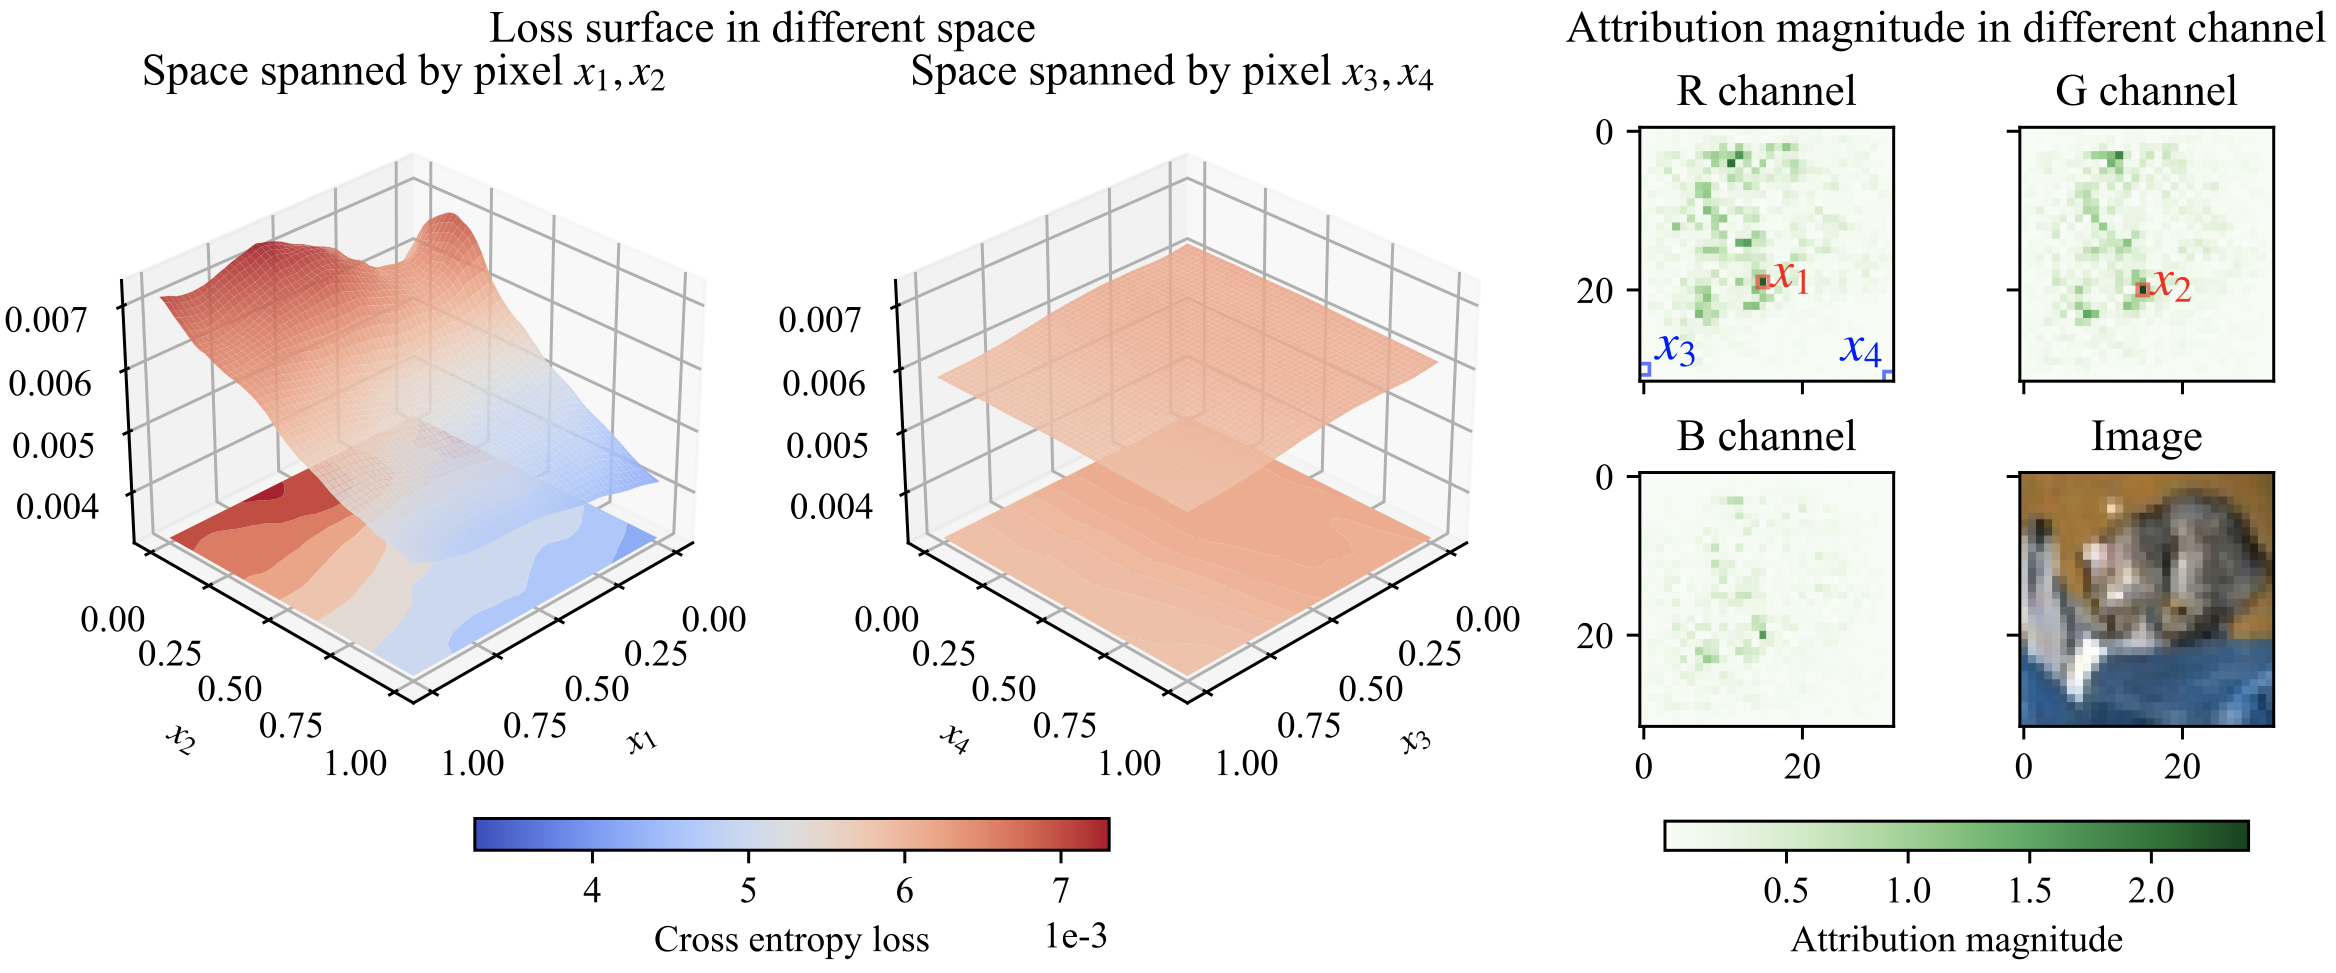
\includegraphics[height = 6cm]{lp-bfgs 1.png}
\end{figure} 
In the context of our project, we would have taken 5 main steps:
\begin{enumerate}
\item Set a working directory and input the model using the load\_model\_tf()
\item Create a function called LBFGS with an objective function (as described above) that minimizes the function maximizing the decrease in image classifier prediction accuracy.
\item Create a for loop that puts each image of the training set through the LBFGS objective function that analyzes pixels and perturbs them, and that ends when the image classifier is 49\% certain on the correct classification of an image. The for loop will calculate the gradient of the objective function for pixels in the image to decide which ones should be perturbed.
\item Use the trained LBFGS algorithm on the test dataset, and put these perturbed images into the classifier.
\item Feed the perturbed test images into the image classifier, and display the test dataset images that fooled the classifier to show an example of successful adversarial attack.
\end{enumerate}

%sub-algorithm three
\subsection{Jacobian-based Saliency Map Attack}
\par In contrast to the L-BFGS method, which inputs an already perturbed image into the image classifier, the Jacobian-based Saliency Map Attack (JBSM) method for adversarial attack uses the output of the image classifier's prediction on an unperturbed image to learn which pixels should be perturbed. The JBSM method turns the image classifier's predicton on the original, untouched image into a Jacobian matrix, which is a matrix of first-order partial derivatives of the variables in a function that describes the behavior of the image classifier with respect to each of the pixels contained in the input image. This Jacobian matrix allows the algorithm to deduce which pixels are the most important in the image classification model's prediction process by creating a saliency map. Building the saliency map involves using the gradient of the function describing the image classifier's behavior to determine how perturbing certain pixels will decrease or increase the accuracy of the image classifier and iterating this process. This saliency map most often takes some type of "heat map" form where pixels in an image are highlighted in different colors based on their importance to the image classifier's recognition of the image's class. After the map is created, the most salient, or important, pixels are selected. These pixels are perturbed and added to the image; the image is fed into the image classifier, and the entire algorithm repeats itself until a satisfactory result is reached.
\begin{figure}[h]
\centering
\caption{Visualization of the Jacobian matrix. A 3-D plot of the matrix of partial derivatives is shown on the right, and level curves are shown on the right.}
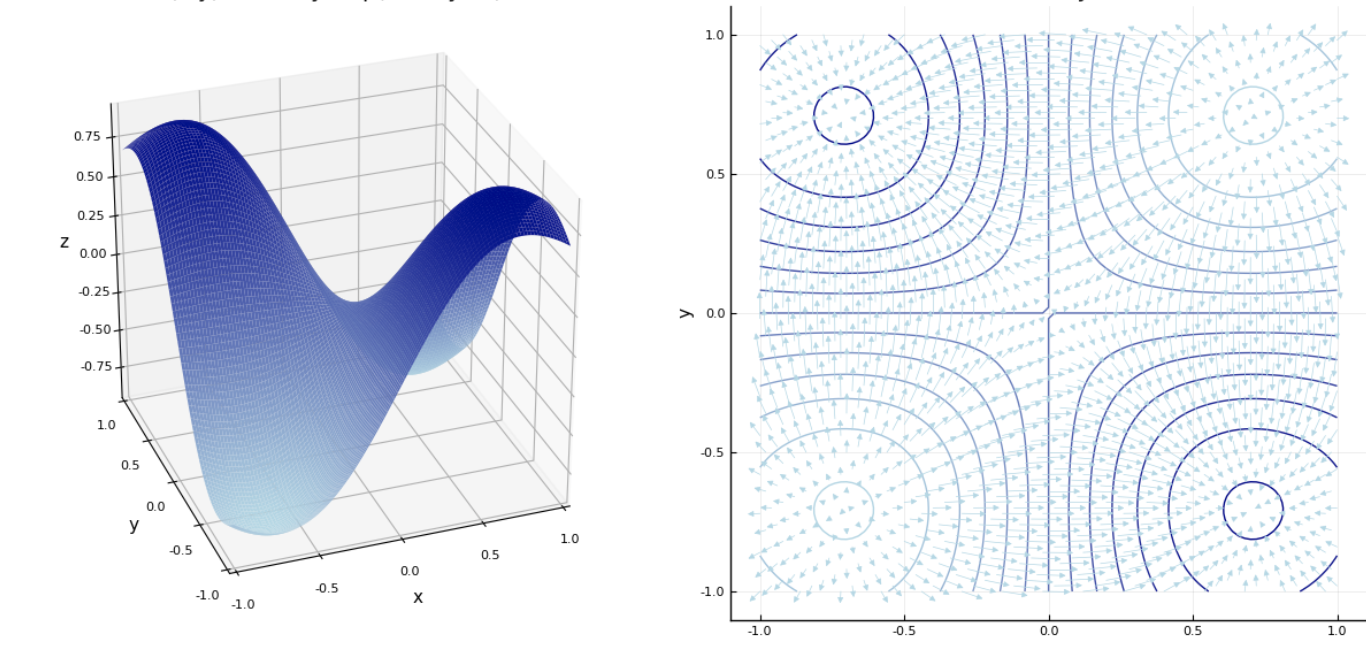
\includegraphics[height = 5.5cm]{jbsm 1.png}
\end{figure} 
\par One useful advantage of the JBSM method is that it perturbs very few features of the image, since pixels are heavily vetted before being selected as perturbation pixels. However, it should be taken into account that the JBSM method may not be the most effective for particularly large networks of data; although the analysis of every single pixel allows for very accurate perturbation placement, it is also computationally taxing.
\begin{figure}[h]
\centering
\caption{Example of the progression of a JBSM algorithm. The first image is the original, unperturbed image, the second is a saliency map describing important pixels, the third image contains the most important pixels discovered after several iterations of the JBSM algorithm, and the fourth image shows the original picture with perturbations added. In this case, the JBSM algorithm has fooled an image classifier into thinking that a number 0 is a number 8.}
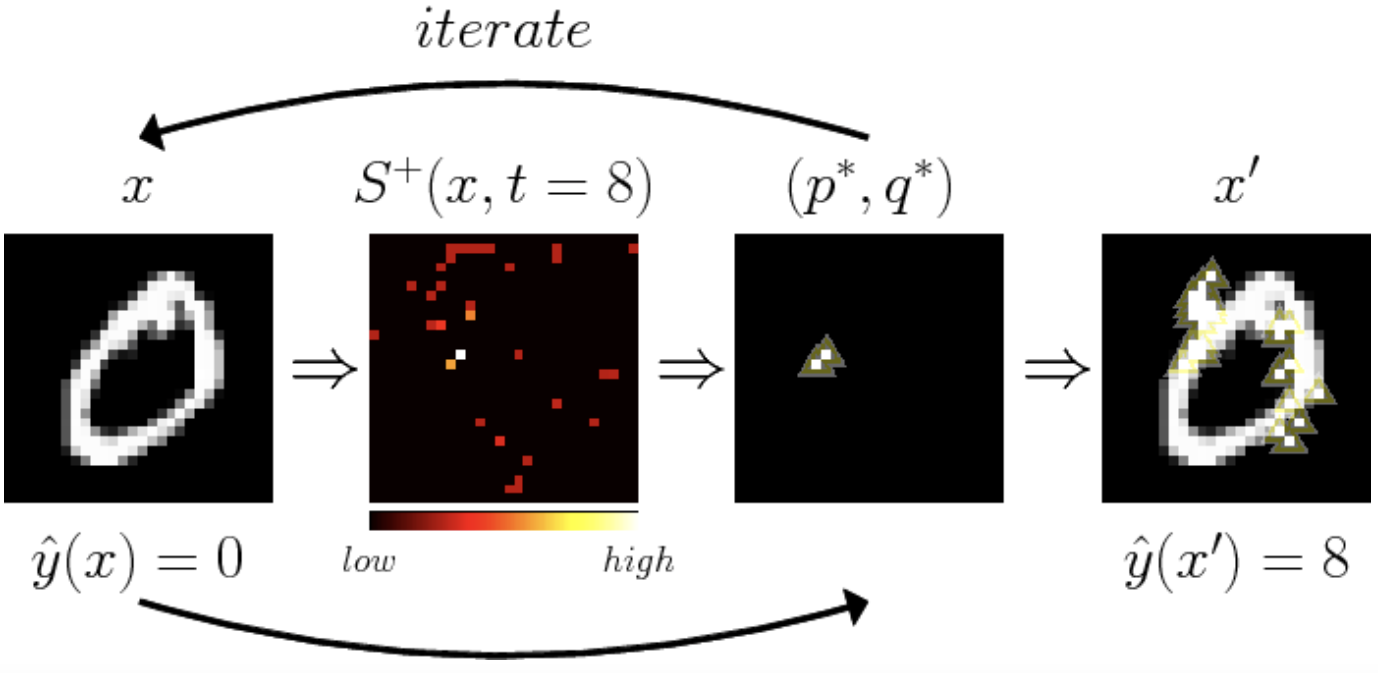
\includegraphics[height = 5.5cm]{jbsm 3.png}
\end{figure}
\newpage
In the context of our project, we would have taken 5 main steps:
\begin{enumerate}
\item Set a working directory and input the model using the load\_model\_tf().
\item Create a function called JBSM that creates the Jacobian matrix from the prediction outputs of the image classifier on an untouched image, and initialize a for loop that puts each image of the training set through the Jacobian matrix and gradient calculations. The for loop will end when the image classifier is 49\% certain on the correct image classification
\item Use the calculations produced to create the saliency map of the image to determine which pixels are the most important, and perturb the pixels selected as the most important ones.
\item Use the trained JBSM algorithm on the test dataset, and feed these perturbed images into the classifier.
\item Display the test dataset images that fooled the classifier to show an example of successful adversarial attack.
\end{enumerate}


\newpage
%sub-algorithm four
\subsection{Deepfool Attack}

%sub-algorithm five:
\subsection{Zeroth-order optimization attack}
\hspace{\parindent} A zeroth order optimization attack is a black box attack, meaning it has access to the inputs and outputs of an image classification model, but it does not have access to the architecture of the model itself.  Most black box attacks make use of a substitute model of the neural network being attacked.  This substitute model is trained using queries input into the target model and their results as training data.  The goal is to build the substitute model and then attack the substitute with a white box attack, with the resulting attack being transferable to the initial target classification model. This type of white box attack uses the known structure of the substitute model to be able to calculate gradients using back propagation (the goal of calculating gradients is to determine which direction to move from the current pixel in order to arrive at a more important pixel).  A zeroth order optimization differs from conventional black box since it does not use a substitute model approximation of the target model.  Instead, the gradient is estimated using a finite difference method of the loss function of the target neural network.  The hessian is also estimated using the same method.  While this method does not give a very numerically accurate estimate of the gradient and hessian, it is good enough to be successful in the context of an attack on an image classifier.  It is worth noting that this method is required to be used in conjunction with stochastic coordinate descent (starting at a random coordinate, finding the gradient and hessian, and calculating the best update to that coordinate) in order to create a computationally feasible solution.  Once a significant coordinate is chosen, it is updated to a new color value using an optimization algorithm for gradient descent called Adam. 
\par The amount of pixels changed, or the amount of noise in the perturbed image is conveniently easily controllable in zeroth order optimization.  This is done by transforming the space that the algorithm is searching for pixels to change into a smaller size.  This is done mainly to decrease the number of calculations required to successfully fool the image classifier, thus decreasing computing resources spent.
\par This algorithm would fool the classifier with subtle (by human visual standards) perturbations of certain pixels located throughout the attack area of an image.  This attack area can be adjusted and increased as necessary to increase the effectiveness at the cost of more computational power being required.  The change to the image is calculated by first evaluating the loss function of the classifier on the target image, then going through the steps described above to arrive at a perturbation.  The noise added to the image is not cohesive in any way, which not only fools the classifier but makes the algorithm harder to defend against than algorithms using an adversarial patch.  The image with this perturbation is then input back into the target classifier. In order to implement this algorithm, we would use the following steps:
\begin{enumerate}
\item Load the model using load\_model\_tf.
\item Input the target image into the image classifier and store output.
\item Define a function to calculate the loss function for a given image based on the output of the image classifier.
\item Define a function to estimate the gradient and hessian based on the result of the loss function.
\item Define a function to calculate the update to a given pixel with the ADAM algorithm, using the estimated gradient and hessian, along with a starting coordinate.
\item Create a transformation of the image desired to be attacked into an attack space of the desired size.
\item Iterate through the above functions to update pixels in the attack space.
\item Transform the attack space with the updates back into it's original dimensions.
\item Input the updated image into the image classifier.

\end{enumerate}

%sources section
\newpage
\section{Weighted Majority Classifier Research}

\par A majority voting classifier is a classifier that takes into account the accuracy of a number of different algorithms and outputs the prediction of the algorithm it deems to be the best. There are two main types of majority voting classifiers that we considered using in the context of this project.
\par A simple majority classifier, in the case of image processing and adversarial attack, would include multiple image classifiers present that each take a vote on one sub-algorithm that is best at fooling the image recognition. From there, the sub-algorithm with the most votes “wins” the vote, and the simple majority classifier will select the set of pixels that the winning sub-algorithm added perturbations to.
\par A weighted majority classifier is slightly different from a simple majority classifier. The first step a weighted majority classifier takes is to distribute weights to each of classifieres themselves. The individual classifiers then place percentage weights on each of the algorithms; at the end, the algorithm with the highest sum of weights is selected as the best one. In the case of our project, sub-algorithms that trick the image classifier into misclassifying the image most often would receive higher weights. The output then consists of the set of pixels that the algorithm with the highest weight perturbed.
\par Our group decided that either one of the two types of majority voting classifiers described above would work equally well for our project. Since we only have one image classifier model, both types of voting classifiers would accomplish the same thing in a very similar way: either by our single classifier voting on one sub-algorithm whose perturbed pixels will become the output (in the case of the hard voting, single majority classifier), or by our single classifier placing the highest weight on a sub-algorithm whose perturbed pixels will become the output (in the case of the soft voting, weighted majority classifier).

\begin{figure}[h]
\centering
\caption{Visual representation of a "hard voting" or simple majority classifier; models vote on the most effective algorithm. Here, algorithm 1 has one the most votes and will be selected as the algorithm.}
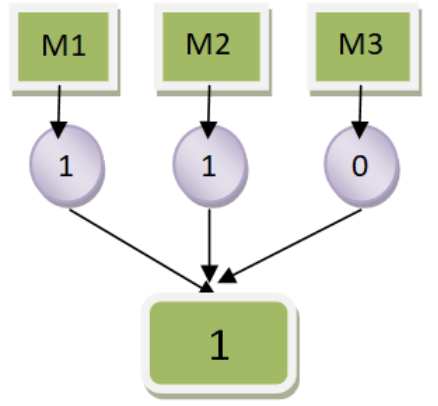
\includegraphics[height = 5.5cm]{hard voting.png}
\end{figure}

\newpage
\begin{figure}[h]
\centering
\caption{Visual representation of a "soft voting", or weighted majority, classifier. }
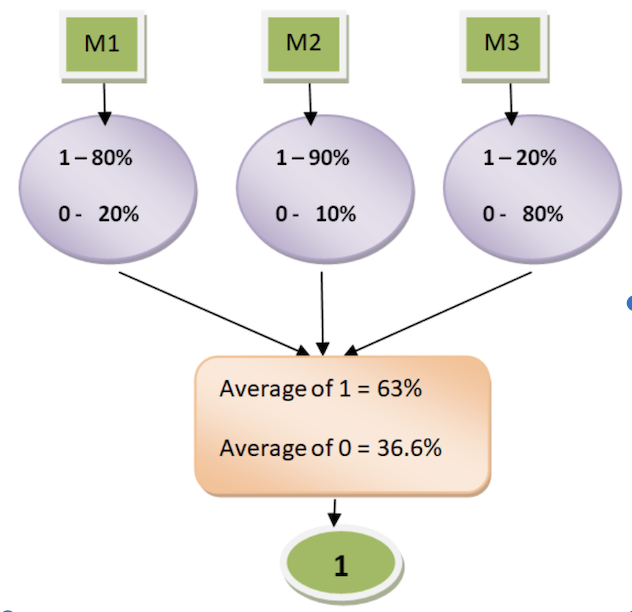
\includegraphics[height = 7cm]{soft voting.png}
\end{figure}


\section{Challenges}

\subsection{Model}
\par One of the challenges that we faced was the uploading of the model files to R. The code given on the video uploaded to Brightspace did not work for some of our teammates, while it did for others. Specifically, some got the “Error in load\_model\_tf(‘./dandelion\_model’) : could not find function ‘load\_model\_tf’” error, while others got “Error: tensorflow.python.framework.errors\_impl.OpError: not an sstable (bad magic number)”. Regarding the first issue, it is important to clarify that the people getting the error tried installing the "tensorflow" package multiple times, along with a extra package called "pillow". These errors prevented 


\subsection{Resources and Documentation}
\par A major challenge our group experienced was in getting Python libraries to function in R using tensorflow.  On multiple group members computers who already had Python installed, the installation of tensorflow from within the RStudio environment encountered several errors.  The main way this challenge was addressed was by uninstalling Python, and allowing R to install Miniconda in order to get tensorflow working.  Once this problem was addressed however, we encountered errors trying to use functions from tensorflow (such as load\_model\_tf) and keras (k\_gradient). Some of these functions worked on some group members computers and not on others.  The best solution we were able to use was to perform all coding and calculations using the computers of those group members who had no issues with the tensorflow and keras packages.  
\par Another challenge stemmed from finding many resources on implementing machine learning and image processing in Python, but very few for how to do so using R.  A major reason this led to confusion for our group is because Python is a heavily object oriented language, while R is classified more as a functional language.  This resulted in confusion and encountering many errors when trying to implement suggestions and solutions into our R code.  We were not able to find a real solution to this issue, which is another main reason why we were not able to construct a working final solution.  One potential solution we considered was to write code in Python, then try to access it using tensorflow, but we quickly discarded this option as all our code for the project was required to be in R.



\subsection{Implementation}
\par A large challenge we faced when attempting to implement the algorithms described above in R was a lack of knowledge on how to actually turn them into code. Although we were able to understand the steps of the algorithms and how they would perform an adversarial attack on the provided image classifier, most of the resources available to us included many complex equations, derivations, and objective functions. 
\par As communicated to us by the instructors, a machine learning algorithm is extremely difficult to create by hand - in this case, it was not a lack of knowledge on the process of the algorithms we researched, but rather a lack of knowledge on how to create the functions that drove the algorithms in R. While we considered simpler options with corresponding libraries in R, such as the rpart package for decision trees or the randomForest package for a random forest model comprised of many decision trees, we did not fully understand how to implement those options in the context of image processing, or how to complete image processing in R. Since our experience with decision trees and random forest models from the last assignment dealt with large datsets that were completely numerical, it was difficult for us to translate that knowledge about classifying positive and negative classes into something applicable to pictures with thousands of pixels.

\newpage
\section{Resources}
\noindent Aung, A. M., Fadila, Y., Gondokaryono, R., \& Gonzalez, L. (n.d.). Building Robust Deep Neural Networks \indent for Road Sign Detection. \\

\noindent Boesch, G. (2023, January 2). What is adversarial machine learning? attack methods in 2023. viso.ai. \indent Retrieved April 28, 2023, from https://viso.ai/deep-learning/adversarial-machine-learning/ \\

\noindent Chen, P.-Y., Zhang, H., Sharma, Y., Yi, J., \& Hsieh, C.-J. (2017). ZOO. \emph{Proceedings of the 10th ACM \indent Workshop on Artificial Intelligence and Security.} https://doi.org/10.1145/3128572.3140448 \\

\noindent Combey, T., Loison, A., Faucher, M., \& Hajri, H. (2020). Probabilistic jacobian-based saliency maps \indent attacks. \emph{Machine Learning and Knowledge Extraction, 2(4), 558–578.} https://doi.org/10.3390/make2040030 \\

\noindent Data Base Camp. (2021, December 17). Explainable AI: Integrated gradients. Data Base Camp. Retrieved \indent April 28, 2023, from https://databasecamp.de/en/ml/integrated-gradients-nlp \\

\noindent Karli, B. T., Sen, D., \& Temizen, A. (2022). Improving Perceptual Quality of Adversarial Images Using \indent Perceptual Distance Minimization and Normalized Variance Weighting. \\

\noindent Kingma, D., \& Ba, J. (n.d.). ADAM: A Method for Stochastic Optimization. \emph{International Conference \indent on Learning Representations.} https://doi.org/https://doi.org/10.48550/arXiv.1412.6980 \\

\noindent LossLandscape. (2022, October 6). Learn about how the A.I, Deep Learning Loss Landscape Project works. \indent LossLandscape. Retrieved April 28, 2023, from https://losslandscape.com/faq/ \\

\noindent Ren, K., Zheng, T., Qin, Z., \& Liu, X. (2020). Adversarial attacks and defenses in Deep Learning. \indent \emph{Engineering, 6(3), 346–360.} https://doi.org/10.1016/j.eng.2019.12.012 \\

\noindent Saeed, M. (2022, March 15). A gentle introduction to Hessian matrices. MachineLearningMastery.com. \indent Retrieved April 28, 2023, from https://machinelearningmastery.com/a-gentle-introduction-to-hessian-\indent matrices/ \\

\noindent Shukla, P. (2022, November 21). Top interview questions on voting ensembles in machine learning. Analytics \indent Vidhya. Retrieved April 28, 2023, from https://www.analyticsvidhya.com/blog/2022/11/top-interview-\indent questions-on-voting-ensembles-in-machine-learning/ \\

\noindent Wiyatno, R., \& Xu, A. (n.d.). Maximal Jacobian-based Saliency Map Attack. 
\end{document}
